\documentclass{ldr-simple-gray}


%------------------------------------------------------------
%首页start
\title{基于稀疏图码的离群值去除}

\subtitle{本科毕业论文(设计)答辩}

\author{庄启源}

\institute[]
{
指导教师:李朋\quad 副教授\\
% 记得改啊,老是有人不改学院……
兰州大学\quad 数学与统计学院
}

\date{\today}

% \logo{
\includegraphics[height=1cm]{lzu_logo.png}}
\titlegraphic{
\includegraphics[height=1.5cm]{lzu_logo.png}}

%首页end
%------------------------------------------------------------

\begin{document}

%封面
\frame{\titlepage}


\begin{frame}{个人信息}

    \begin{itemize}
        % 记得改啊
        \item 姓名:庄启源
        \item 指导教师:李朋\quad 副教授
        \item 专业:数学(基础理论班)
        \item 邮箱:zhuangqy20@lzu.edu.cn
    \end{itemize}

    \qquad \noindent\rule[0.25\baselineskip]{0.9\textwidth}{1pt}


    % \begin{itemize}
    %     \item 本科:2016-2020 \quad 兰州大学 \quad 物理科学与技术学院
    %     \item 硕士:2020-至今 \quad 兰州大学 \quad 物理科学与技术学院
    % \end{itemize}

    % \qquad \noindent\rule[0.25\baselineskip]{0.9\textwidth}{1pt}

    \begin{itemize}
        \item 论文题目:基于稀疏图码的离群值去除
        \item 关键词:压缩感知;离群值;稀疏信号恢复;稀疏图码
    \end{itemize}
\end{frame}

% 要把今天讲的研究背景、主要结果、价值和意义(贡献点)讲清楚

\section{研究背景}

\begin{frame}{相关解释}
    \begin{itemize}
        \item \textbf{主要内容:无噪声情形下,当观测信号存在少量离群值时稀疏信号的精确恢复。}
        \item \textbf{压缩感知问题:}对一个稀疏信号$\mathbf{x} \in \mathbb{R}^N$,
        使用一个测量矩阵$\mathbf{A}$采样后得到一个观测向量$\mathbf{y} \in \mathbb{R}^M$,
        再由该观测值估计初始信号。
        \item \textbf{拓展问题:}考虑观测值中出现离群值的情况,观测过程可表示为
        \begin{equation*}
            \mathbf{y} = \mathbf{Ax} + \mathbf{f}, 
        \end{equation*}
        其中$\left | \mathrm{supp} (\mathbf{f}) \right | = T = \eta M << M$,
        且$\mathbf{f}$中非零元素的分布方差显著大于$\mathbf{x}$中的非零元素。
    \end{itemize}
\end{frame}


\begin{frame}{现有研究}
    次线性时间的支撑集恢复
    \begin{itemize}
        \item 目的:测量值数目$M$尽可能小;恢复信号所需的时间复杂度尽可能小。
        \item Li、Yin\footfullcite{8733902}等人建立了一种基于稀疏图码的压缩感知框架,能够在无噪声情况下,
        用$2K$次测量精确地恢复任意稀疏度为$K$的信号,解码时间复杂度达到$O(K)$。
        \item Bakshi、Jaggi\footfullcite{7185441}等人提出的SHO-FA算法使有噪声情形下的信号恢复
        仅需$O(K)$次测量且编码解码时间复杂度分别为$O(N)$和$O(K)$。
    \end{itemize}
    % \begin{figure}
    %     \subfigure[2nm、10-160\%\footfullcite{Zhang2011}]{
    %         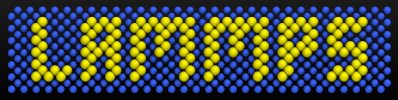
\includegraphics[width=0.28\textwidth]{lammps.png}
    %      }
    %      \subfigure[5nm、50-350\%\footfullcite{Zhang2011}]{
    %          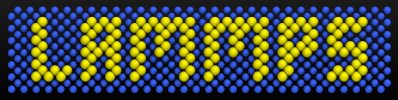
\includegraphics[width=0.36\textwidth]{lammps.png}
    %       }\\
    %     \subfigure[20nm、25-45\%\footfullcite{Zhang2011}]{
    %         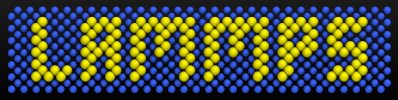
\includegraphics[width=0.4\textwidth]{lammps.png}
    %      }
    % \end{figure}
\end{frame}

\begin{frame}{稀疏图码}
    \begin{figure}
        \centering
        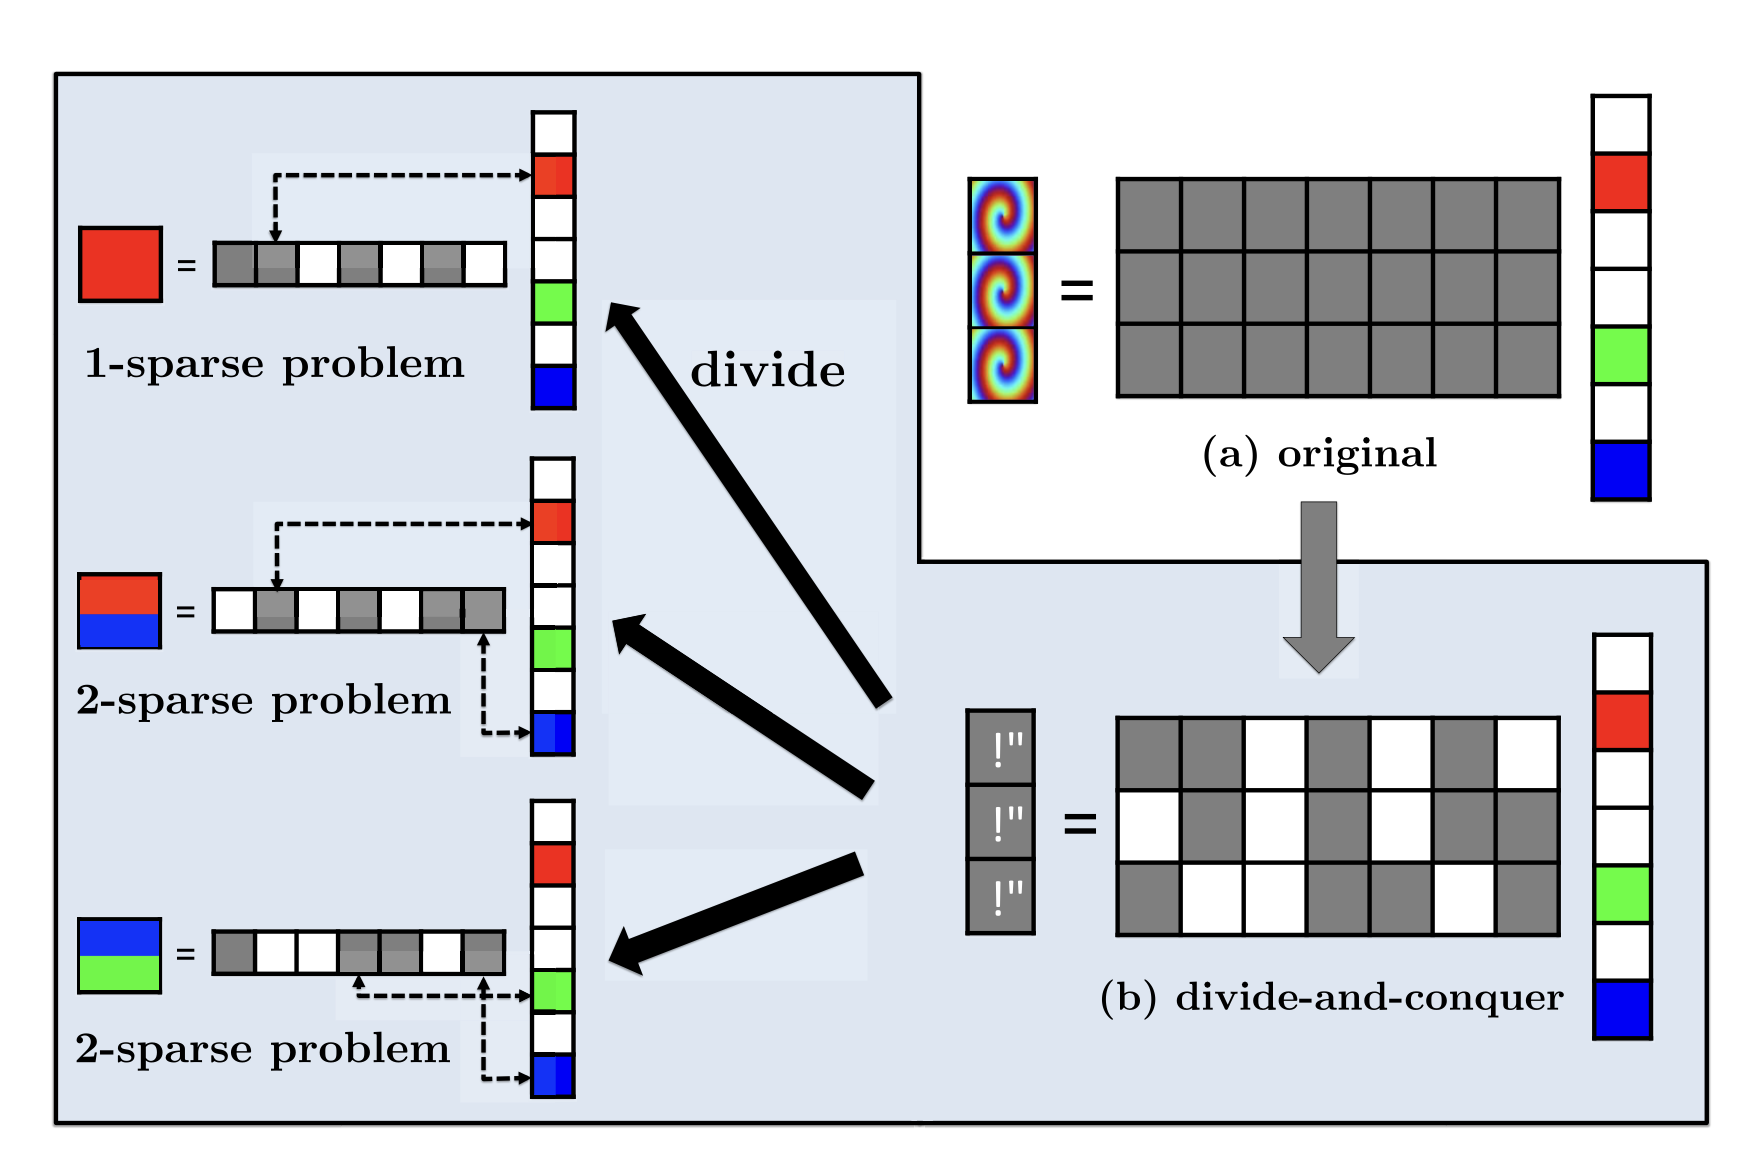
\includegraphics[width=0.6\textwidth]{d_n_c.png}
    \end{figure}
    分治法:设计的测量矩阵将稀疏度为3的恢复问题分解为多个稀疏度小于3的子问题,再逐步剥离解决问题。
\end{frame}


\begin{frame}{存在的问题}
    \begin{itemize}
        \item 现有的基于稀疏图码的信号重构策略能快速精确恢复信号,但无法解决存在离群值时的问题。
        \item 能够解决离群值问题的算法无法达到次线性时间复杂度。
    \end{itemize}
\end{frame}

\section{研究内容}

\begin{frame}{测量矩阵的设计}
    
    \begin{columns}
        \column{0.6\textwidth}
        正则度为2的左正则二部图邻接矩阵$\mathbf{H}$\\
        右图表示$\mathbf{y} = \mathbf{Hx}$
        \begin{itemize}
            \item \textbf{零节点}:不包含任何非零元素的右节点,如$y_1$。
            \item \textbf{单节点}:仅包含一个非零元素的右节点,如$y_5$。
            \item \textbf{多节点}:包含一个以上非零元素的右节点,如$y_2$。
        \end{itemize}
        \column{0.5\textwidth}
        \begin{figure}
            \centering
            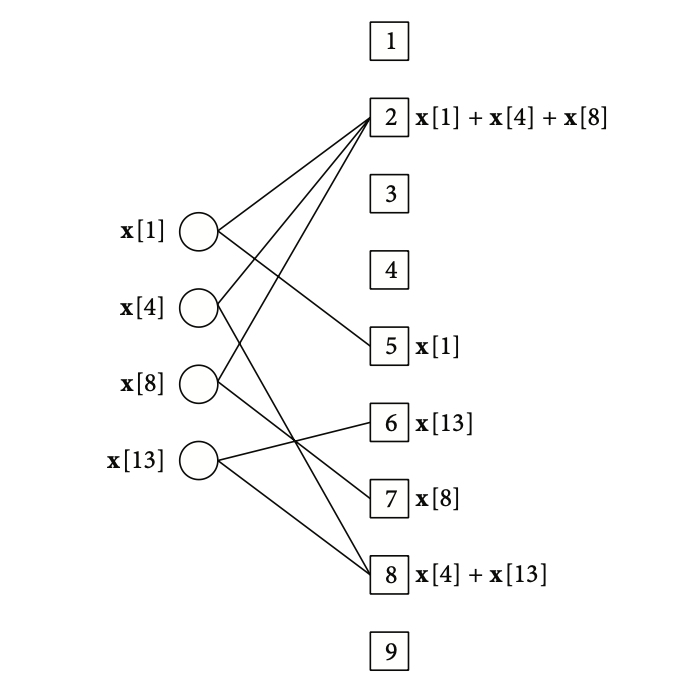
\includegraphics[width=1\textwidth]{bip_g.png}
        \end{figure}
        
    \end{columns}

\end{frame}

\begin{frame}{测量矩阵的设计}
    \begin{itemize}
        \item \textbf{检测矩阵}$\mathbf{S}$:
        \begin{equation*}
            \mathbf{S}=
            \left[
                \begin{array}{ccccccc}
                    1 & 1 & 1  & 1 & 1 & \dots & 1 \\
                    1 & W & W^2 & W^3 & W^4 & \dots & W^{15}
                \end{array}
                \right],
            \label{S}
        \end{equation*}
        其中$W = e^{i \frac{2\pi}{N}}$是一个$N$次单位根,
        $\mathbf{S}$是一个$N \times N$的DFT矩阵的前两行。
        \item \textbf{行张量算子} $\boxtimes$:
        \begin{equation*}
            \mathbf{A} = \mathbf{H} \boxtimes \mathbf{S} = \left[\mathbf{h}_0 \otimes \mathbf{s}_0 , \cdots , \mathbf{h}_{N-1} \otimes \mathbf{s}_{N-1} \right],
        \end{equation*}
        其中$\otimes$是一个克罗内克积。
    \end{itemize}
\end{frame}

\begin{frame}{测量矩阵例子}
    \begin{equation*}
        \mathbf{H} = 
        \left[
            \begin{array}{ccccccc}
                1 & 1 & 0 & 1 & 0 & 1 & 0 \\
                0 & 1 & 0 & 1 & 0 & 0 & 1 \\
                1 & 0 & 0 & 1 & 1 & 0 & 1
            \end{array}
        \right], 
    \end{equation*}
    \begin{equation*}
        \mathbf{S} = 
        \left[
            \begin{array}{ccccccc}
                1 & 1 & 1  & 1 & \dots & 1 \\
                1 & W & W^2 & W^3 & \dots & W^6
            \end{array}
        \right].
    \end{equation*}
    $\Rightarrow$
    \begin{equation*}
        \mathbf{H} \boxtimes \mathbf{S} = 
        \left[
            \begin{array}{ccccccc}
                1 & 1 & 0 & 1 & 0 & 1 & 0\\
                1 & W & 0 & W^3 & 0 & W^5 & 0\\
                0 & 1 & 0 & 1 & 0 & 0 & 1 \\
                0 & W & 0 & W^3 & 0 & 0 & W^6 \\
                1 & 0 & 0 & 1 & 1 & 0 & 1\\
                1 & 0 & 0 & W^3 & W^4 & 0 & W^6
            \end{array}
        \right].
    \end{equation*}
\end{frame}
% \begin{frame}{做了啥?}
%     复杂布局:上下布局、左右分栏

%     \begin{columns}
%         \column{0.7\textwidth}
%     \begin{itemize}
%         \item 11111
%         \item 22222
%         \item 33333
%     \end{itemize}

%     \begin{figure}
%         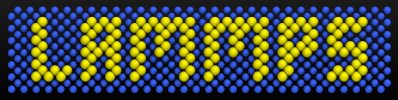
\includegraphics[width=0.4\textwidth]{lammps.png}
%         \caption{图图图}
%     \end{figure}
%     \column{0.3\textwidth}

%     \begin{figure}
%         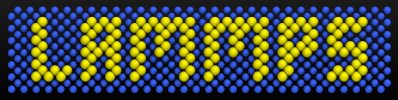
\includegraphics[angle=80, width=0.4\textwidth]{lammps.png}
%         \caption{我转}
%     \end{figure}
%     \end{columns}

% \end{frame}

\begin{frame}{节点类型检测}
    \textbf{测量对}:二维向量$\mathbf{y}_r = [y_r[0], y_r[1]]^T$,例如
    $\mathbf{y}_5 = x[1] \times
    \left[
        \begin{array}{c}
            1 \\ W
        \end{array}
    \right]$.\\
    \textbf{比值检测}:
    \begin{equation*}
        \label{k}
        \hat k = \frac{\angle y_r[1] / y_r[0]}{2 \pi / N}.
    \end{equation*}
    \begin{itemize}
        \item \textbf{零节点对}:测量对是一个全0向量,即$\mathbf{y}_r = \mathbf{0}$.
        \item \textbf{单节点对}:$\hat k$为整数。
        \item \textbf{多节点对}:$\hat k$不为非零整数或两个元素不同模$|y_2[1]| \neq |y_2[0]|$。
        例如,
        \begin{equation*}
            \hat k = \frac{\angle y_2[1] / y_2[0]}{2 \pi / 16} = 4.85995. 
        \end{equation*}
    \end{itemize}
\end{frame}

\begin{frame}{剥离解码步骤}
    \begin{itemize}
        \item 找到所有零节点(对)并剥离所有相应的左右节点对和边。
        \item 选取二部图中所有使得右节点度数为1的边(找到所有单节点),恢复对应左节点。
        \item 去除(剥离)所有这些边以及与之对应的左右节点对。
        \item 去除(剥离)上一步骤中剥离的左节点的其他未被剥离的边。
        \item 找到上一步骤中去除的左节点连接的所有右节点,将这些左节点的值从右节点的值中减去。
    \end{itemize}
    \begin{figure}
        \centering
        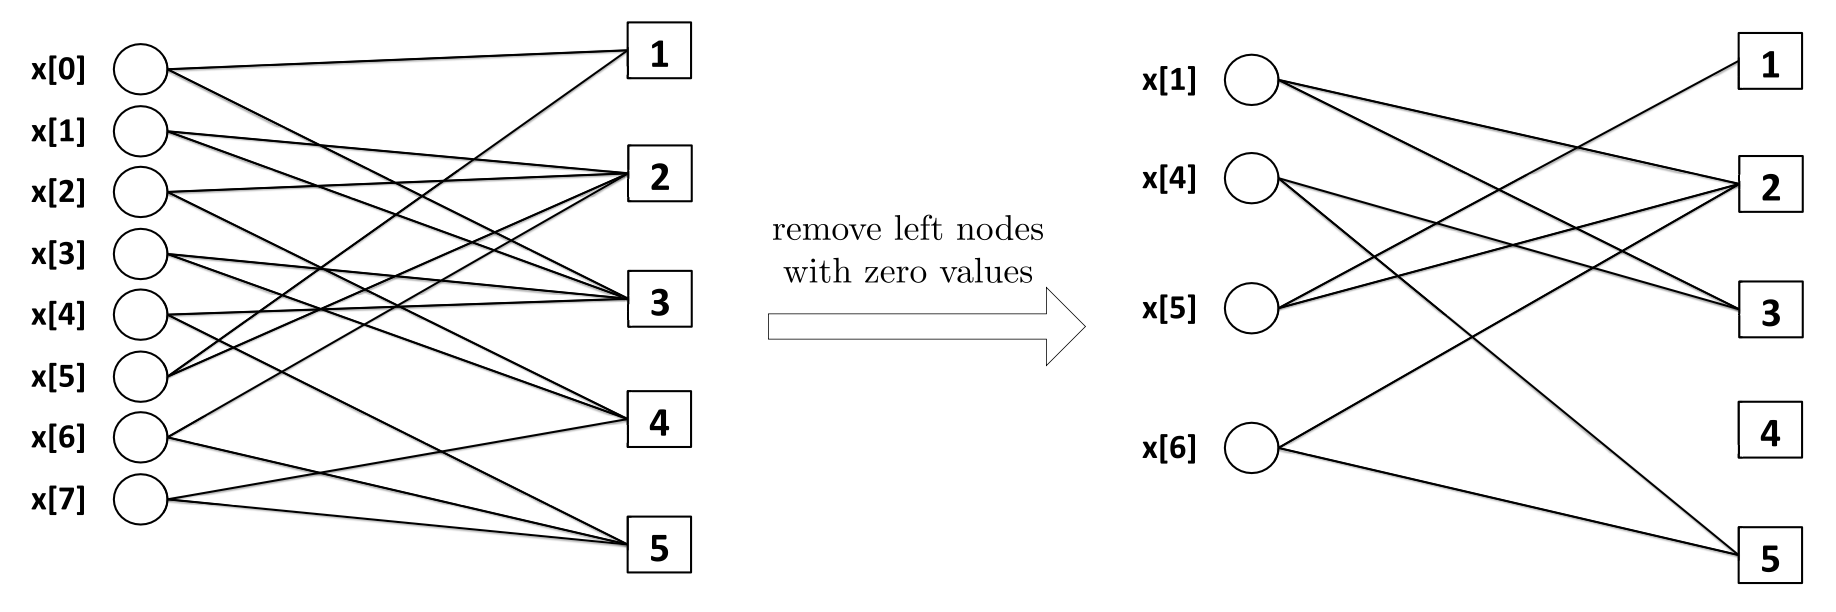
\includegraphics[width=0.8\textwidth]{peeling.png}
    \end{figure}
\end{frame}

\begin{frame}{离群值去除}
    把$\mathbf{y}$的有效非零元素限制在一个指标集
    \begin{equation*}
        S = \{s: |y_s| < \alpha \theta_p (\{|y_j| : j \in \mathrm{supp} (\mathbf{y})\})\}
    \end{equation*}
    上,其他指标的对应元素全部设为0。
    \begin{algorithm}[H]
        \caption{离群值去除算法\label{Alg:outliers_removal}}
        \hspace*{0.02in} {\bf 输入:} 
        观测值 $\mathbf{y} \in \mathbb{C}^{2R}$(测量对形式),常数$\alpha$和$p$。
        \begin{algorithmic}[1]
            \State 首先计算得到$\mathbf{y}$的非零元素模的分位数$q = \theta_p (\{|\mathbf{y}_j[0]|: \mathbf{y}_j[0] \neq 0, \mathbf{y}_j \in \mathbf{y}\})$;
            \For{$r = 1$ to $R$}
                \If{$|\mathbf{y}_r [0]| > \alpha \cdot q$}
                    \State 将$\mathbf{y}_r$抹去为$\mathbf{0}$向量;
                \EndIf
            \EndFor
        \end{algorithmic}
    \end{algorithm}
\end{frame}

\begin{frame}{PAMQ算法}
    \begin{itemize}
        \item \textbf{两阶段算法}:先去除离群值,再恢复信号。在离群值去除过程中,我们把分位数乘上一定倍率作为分割点;
        在信号恢复中,我们应用稀疏图码中的剥离解码方法。\\
        因此我们把这一算法命名为PAMQ(Peeling after Multiplied Quantile)算法。
        \item \textbf{创新点}:将基于稀疏图码的信号恢复算法应用到存在离群值场景,
        与自定义的离群值去除技巧结合,形成全新有效算法。
    \end{itemize}
\end{frame}

\section{数值结果}

\begin{frame}{实验设置}
    评价指标\textbf{精确恢复率}:
    多次重复实验中恢复结果误差err < thr\_err的次数与总实验次数的比值。
    其中,
    \begin{equation*}
        err=\frac{||{\mathbf{x} - \hat{\mathbf{x}}}||_2}{||\mathbf{x}||_2},
    \end{equation*}
    thr\_err = $10^{-2}$或$10^{-7}$。
    \begin{itemize}
        \item 初始稀疏信号$\mathbf{x} \in \mathbb{R}^{200}$且
        其中非零元素$x_i \sim N(0,1)$;
        \item 离群向量$\mathbf{f}$中的非零元素$f_j \sim N(0,100)$;
        \item 编码矩阵$\mathbf{H}$为每列有且仅有三个1的矩阵,即正则度为3的左正则二部图邻接矩阵;
        \item 检测矩阵$\mathbf{S}$为$N \times N$的DFT矩阵前两行。
    \end{itemize}
\end{frame}

\begin{frame}{信号恢复效率}
    \begin{table}[H]
        \centering
        \caption{不同测量次数下的恢复效率}
        \resizebox{\textwidth}{!}{
        \begin{tabular}{ccccccc} % 控制表格的格式,可以是l,c,r
            \toprule
            测量值数目$M$ & 10  & 20  & 40  & 80 & 100 & 120 \\
            \toprule
            精确恢复率 & 70.0\% & 84.5\% & 90.5\%  & 92.5\% & 95.5\% & 95.0\% \\
            \midrule
            平均用时(毫秒) & 48.55 & 79.25 & 89.70 & 95.40 & 115.25 & 126.50 \\
            \bottomrule
        \end{tabular}}
        \label{effeciency}
    \end{table}

    \begin{table}[H]
        \centering
        \caption{不同信号稀疏度下的恢复效率}
        \begin{tabular}{cccccc} % 控制表格的格式,可以是l,c,r
            \toprule
            稀疏度$K$ & 1  & 2  & 3  & 4 & 5\\
            \toprule
            精确恢复率 & 98.0\% & 95.4\% & 92.2\%  & 91.8\% & 88.8\%\\
            \midrule
            平均用时(毫秒) & 124.0 & 129.0 & 129.6 &  125.4 & 130.4\\
            \bottomrule
        \end{tabular}
        \label{diff_sprs}
    \end{table}

\end{frame}

\begin{frame}{算法参数取值的影响}
    \begin{figure}[H]
        \centering
        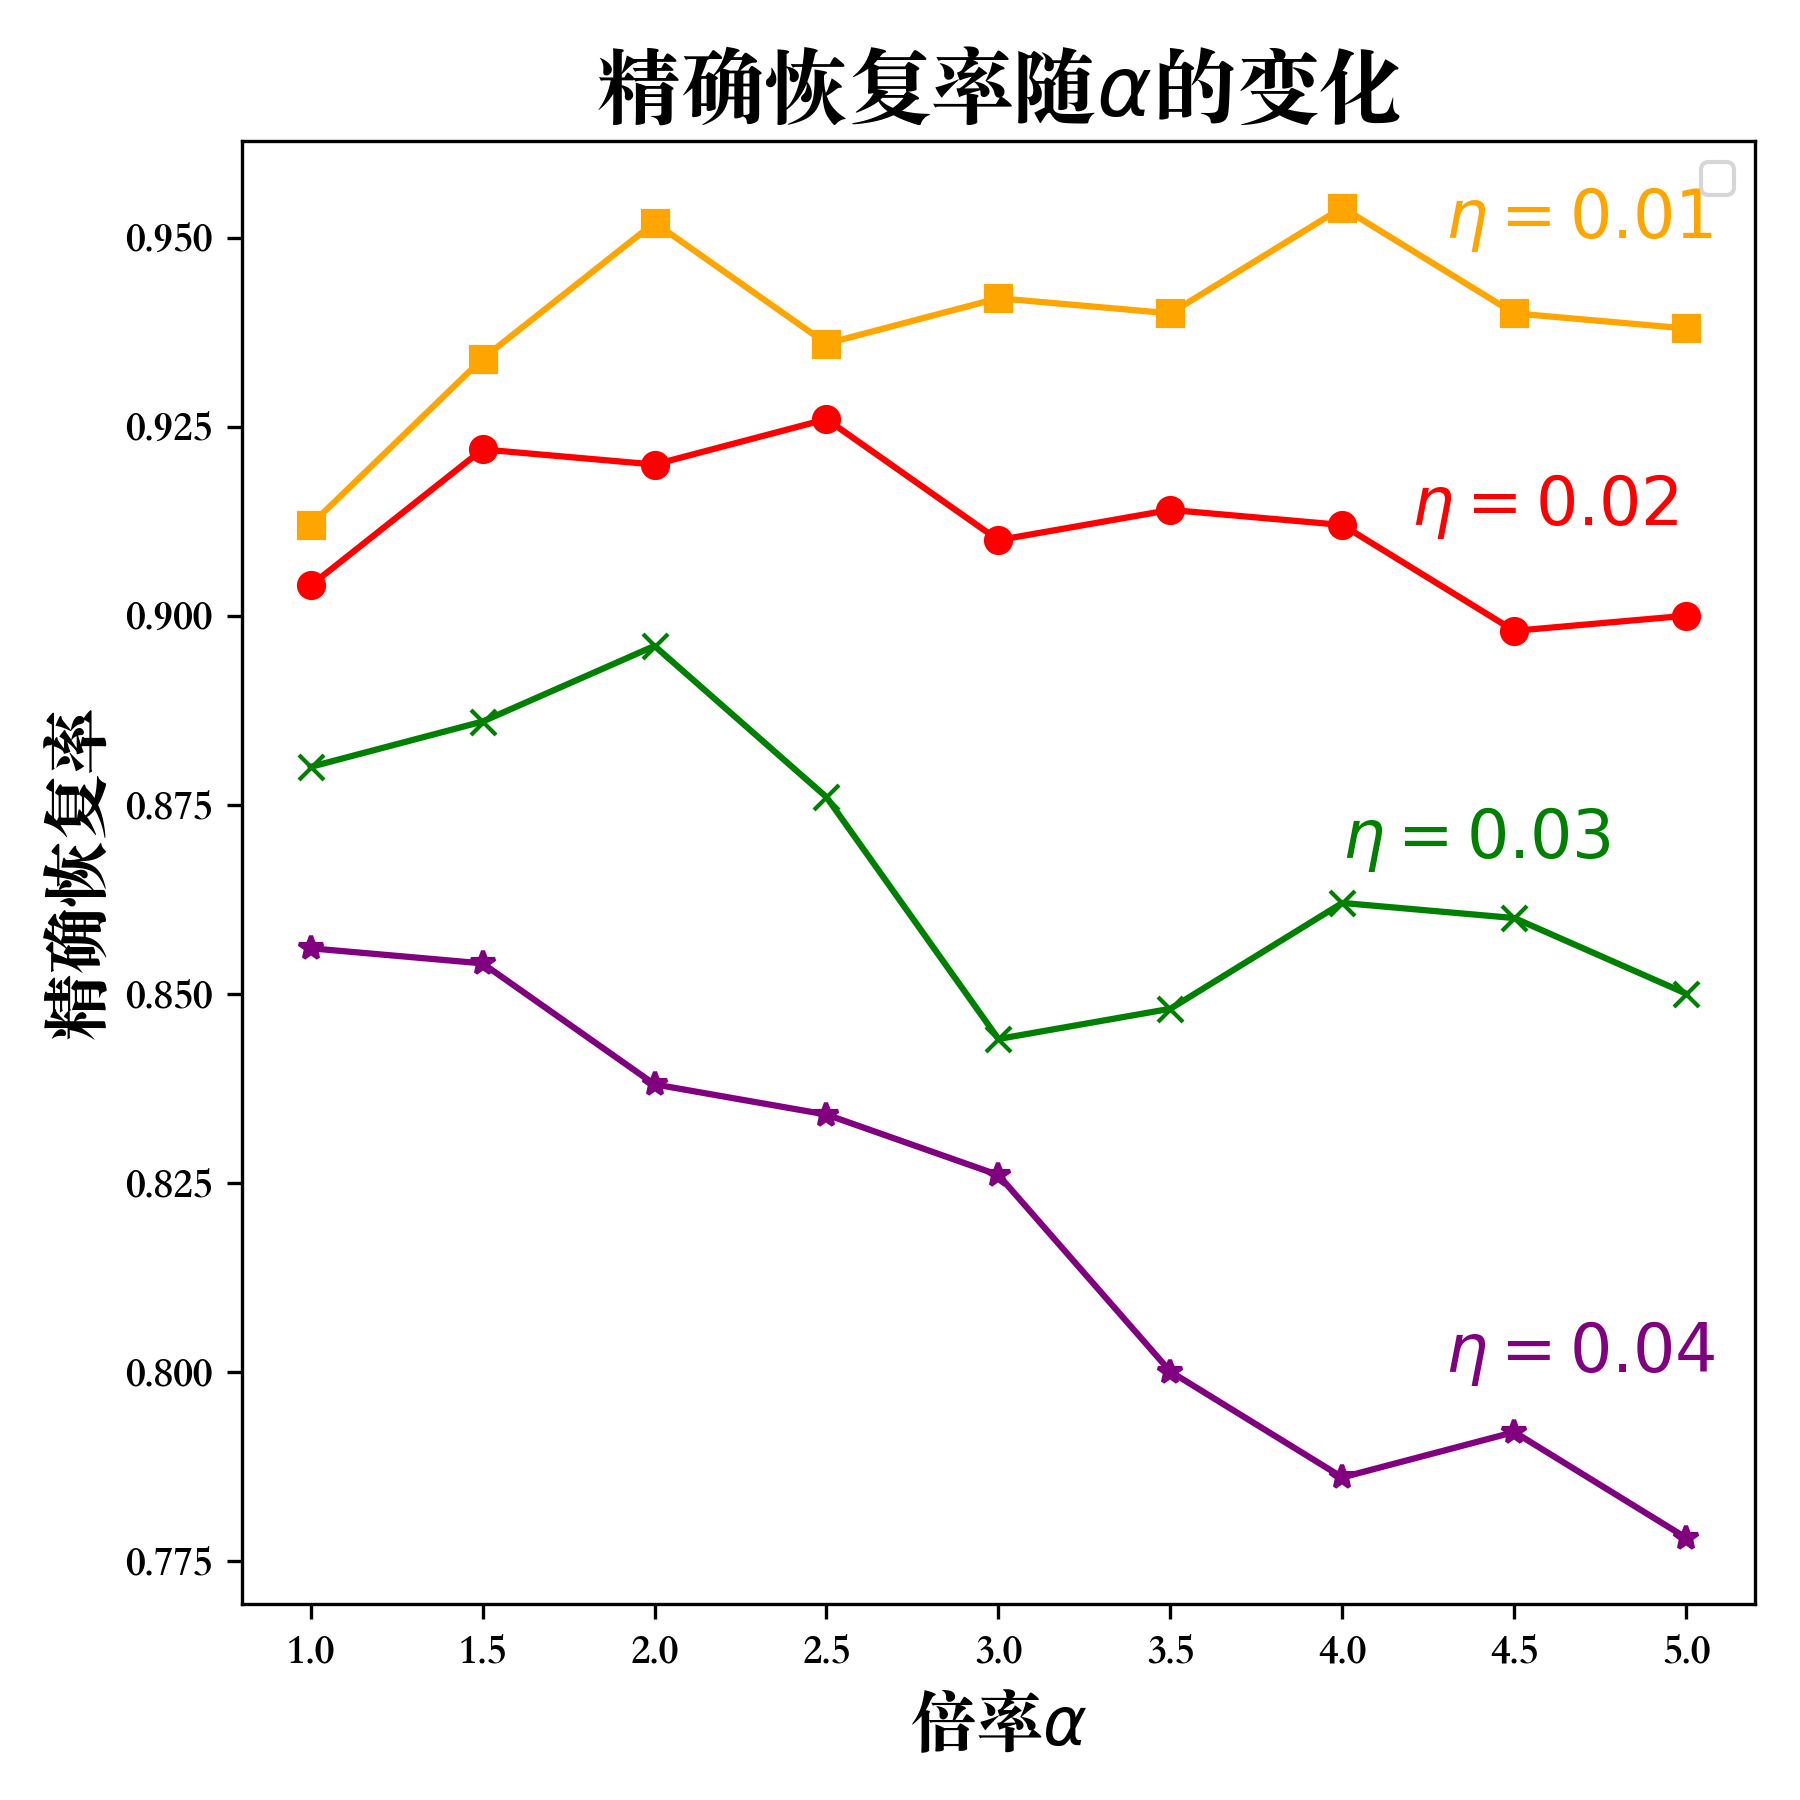
\includegraphics[width=0.5\textwidth]{figures/diff_alpha.png}
        \caption{不同离群值比例下的恢复效果随算法参数变化展示。
            图中横坐标表示不同的倍率$\alpha$,纵坐标表示精确恢复率,
            四条曲线分别表示离群值比例$\eta$取$1\%, 2\%, 3\%, 4\%$的情形。
            }
        \label{fig_diff_alg}
    \end{figure}
\end{frame}

\begin{frame}{与其他算法的比较}
    选取对比算法为$\ell_1$-PLAD算法(Penalized Least Absolute Deviation)。
    \begin{equation*}
        \min_{\mathbf{x} \in \mathbb{R}^N}{||\mathbf{y} - \mathbf{Ax}||_1 + \lambda ||\mathbf{x}||_1}
    \end{equation*}
    其中$\mathbf{A}$是一个$M \times N$的高斯测量矩阵。

    \begin{table}[H]
        \centering
        \caption{PAMQ算法与PLAD算法的对比}
        \resizebox{\textwidth}{!}{
        \begin{tabular}{cccccc} % 控制表格的格式,可以是l,c,r
            \toprule
            应用算法 & PAMQ  & \eqrm{PLAD_{\lambda = 0.006}}  & \eqrm{PLAD_{\lambda = 0.007}}  & \eqrm{PLAD_{\lambda = 0.008}} & \eqrm{PLAD_{\lambda = 0.009}}\\
            \toprule
            $\eta = 0.02$ & 92.0\% & 78.2\% & 94.6\% & 91.2\%  & 79.8\%\\
            \midrule
            $\eta = 0.03$ & 89.8\% & 47.8\% & 66.4\% & 92.2\%  & 92.0\%\\
            \toprule
            平均用时(毫秒) & 129.0 & 1729.9 & 1268.3 & 1692.2 &  2374.5\\
            \bottomrule
        \end{tabular}}
        \label{diff_algs}
    \end{table}
\end{frame}

\section{结论}

\begin{frame}{价值和意义}
    \begin{itemize}
        \item 恢复仅需极短的CPU时间,速度是PLAD算法的十倍。
        \item 能够适应少量的离群值,恢复比PLAD更精确,能够使err $< 10^{-7}$。
        \item 对不同的情况更具一般性和稳定性,不会因算法参数($\alpha, p$)变化产生极大波动。
    \end{itemize}
\end{frame}
% \begin{frame}{价值和意义}
    
%     \begin{itemize}
%         \item 给出了……,预测了……。
%         \item 相比其他,此材料\textcolor{Logo2}{多厉害、多厉害、……}
%         \item 为……提供了解决思路。
%     \end{itemize}
    
% \end{frame}

% \section{博士计划}

% \begin{frame}{计划往往是不去做、或无法完成的}

%     找女朋友,找女朋友,找女朋友\footfullcite{Zhang2011}

%     找女朋友,找女朋友,找女朋友\footfullcite{Zhang2011}

%     找女朋友,找女朋友,找女朋友\footfullcite{Zhang2011}

%     \begin{figure}[H]
%         \centering
%         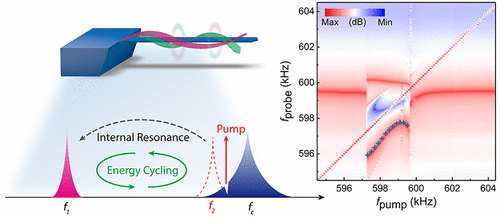
\includegraphics[width=0.47\textwidth]{2022-04-16-06-26-14.png}
%     \end{figure}
%     重要的事情说9遍,九九归一、大彻大悟
% 
% \end{frame}


\begin{frame}{\quad}
\begin{center}
       \zihao{2} 谢\quad 谢!
\end{center}

\end{frame}

\end{document}